\section{Problem Definition}

In our discussion, TV watching sequence refers to a channel switching sequence generated from a TV. The switching records in the
sequence are arranged according to the switching in time. And between any two switching records, the switching out time of the first
records may or may not be the same as the switching out time. If the two times are different, it means the TV isn't watched by 
any users in this duration. An illustration is depicted in table \ref{tbl:1}.

\begin{table}[!htbp]
\centering
\begin{tabular}{|c||c||c|}
\hline
Channel & Start Time & End Time\\
\hline
Channel 1 & 22:00:00 & 22:00:30\\
\hline
Channel 2 & 22:30:40 & 23:00:00\\
\hline
Channel 3 & 23:00:00 & 23:30:00\\
\hline
... & ... & ... \\
\hline
Channel 1 & 23:45:00 & 23:48:00\\
\hline
\end{tabular}
\caption{TV Watching Sequence Example}
\label{tbl:1}
\end{table}

Then given a TV watching sequence, the problem is defined as finding how many users have watched the TV and finding the corresponding
watching record for each of them. Figure \ref{fig:1} illustrates the problem.

\begin{figure}[htbp]
\centering
\includegraphics[width=2.5in]{probdef.eps}
\caption{Problem Illustration}
\label{fig:1}
\end{figure}
